% Paquets généraux
\documentclass[a4paper,12pt,titlepage]{article}
\usepackage[T1]{fontenc}
\usepackage[utf8]{inputenc}
\usepackage[french]{babel}
\usepackage[gen]{eurosym}
%\usepackage[dvips]{graphicx}
\usepackage{fancyhdr}
\usepackage{pdfpages} 
\usepackage{multido}
\usepackage{hyperref}
%\usepackage{textcomp}
%\usepackage{aeguill}
\usepackage{schemabloc}
\usepackage[bitstream-charter]{mathdesign}

\newcommand{\id}{54}
\newcommand{\nom}{Liaisons mécaniques}
\newcommand{\sequence}{04}
\newcommand{\num}{01}
\newcommand{\type}{TP}
\newcommand{\descrip}{Modélisation d'un solide. Comportement des liaisons mécaniques. Modéliser les mécanismes du laboratoire par un schéma cinématique, paramétré.}
\newcommand{\competences}{A3-C4: Analyse d'architecture et de comportement \\ &  Mod1-C1: Isolement d'un solide ou d'un système de solides \\ &  Mod2-C10-1: Modèle de solide indéformable \\ &  Mod2-C11: Modélisation géométrique et cinématique des mouvements entre solides indéformables \\ &  Mod2-C12: Modélisation cinématique des liaisons entre solides \\ &  Mod2-C15: Modélisation des actions mécaniques \\ &  Rés-C6: Utilisation d'un solveur ou d'un logiciel multi physique \\ &  Com1-C1: Différents descripteurs introduits dans le programme \\ &  Com2-C4: Outils de communication}
\newcommand{\nbcomp}{9}
\newcommand{\systemes}{Plateforme Stewart}
\newcommand{\systemessansaccent}{Plateforme Stewart}
\newcommand{\ilot}{2}
\newcommand{\ilotstr}{02}
\newcommand{\dossierilot}{\detokenize{Ilot_02 Plateforme Stewart}}
\newcommand{\imageun}{Plateforme}

\newcommand{\urlsysteme}{\href{https://www.costadoat.fr/systeme/57}{Ressources système}}
\newcommand{\matlabsimscape}{\href{https://github.com/Costadoat/Sciences-Ingenieur/raw/master/Systemes/Plateforme Stewart/Plateforme_Stewart_Simscape.zip}{Modèle Simscape}}
\newcommand{\solidworks}{\href{https://github.com/Costadoat/Sciences-Ingenieur/raw/master/Systemes/Plateforme Stewart/Plateforme_Stewart_Solidworks.zip}{Modèle Solidworks}}
\newcommand{\edrawings}{\href{https://github.com/Costadoat/Sciences-Ingenieur/raw/master/Systemes/Plateforme Stewart/Plateforme_Stewart.EASM}{Modèle eDrawings}}
\newcommand{\test}{Stewart_param1}
\newcommand{\testi}{Stewart_param2}
\newcommand{\testii}{Stewart_param3}
\newcommand{\testiii}{Stewart_param4}
\newcommand{\testiiii}{Stewart_euler}

\newcommand{\auteurun}{Renaud Costadoat}
\newcommand{\auteurdeux}{Françoise Puig}
\newcommand{\institute}{Lycée Dorian}


\usepackage{color}
\usepackage{xcolor}
\usepackage{colortbl}
\usepackage{helvet}
\renewcommand{\familydefault}{\sfdefault}
\usepackage{amsfonts}
\usepackage{amsmath}
%\usepackage{xspace}
\usepackage{varioref}
\usepackage{tabularx}
%\usepackage{floatflt}
\usepackage{graphics}
\usepackage{wrapfig}
\usepackage{textcomp}
\usepackage{tikz}
\usepackage{wrapfig}
\usepackage{gensymb}
\usepackage[european]{circuitikz}
\usetikzlibrary{babel}
\usepackage{ifthen}
\usepackage{cancel}
\usepackage{etoolbox}
\usepackage{multirow}
%\usepackage{boxedminipage}
\definecolor{gris25}{gray}{0.75}
\definecolor{bleu}{RGB}{18,33,98}
\definecolor{bleuf}{RGB}{42,94,171}
\definecolor{bleuc}{RGB}{231,239,247}
\definecolor{rougef}{RGB}{185,18,27}
\definecolor{rougec}{RGB}{255,188,204}%255,230,231
\definecolor{vertf}{RGB}{103,126,82}
\definecolor{vertc}{RGB}{220,255,191}
\definecolor{forestgreen}{rgb}{0.13,0.54,0.13}
\definecolor{blcr}{rgb}{0.59,0.69,0.84}
\definecolor{blfr}{rgb}{0.32,0.51,0.75}
\definecolor{orfr}{rgb}{0.90,0.42,0.15}
\definecolor{orcr}{rgb}{0.90,0.65,0.50}
\definecolor{orangef}{rgb}{0.659,0.269,0.072}
\definecolor{orange}{rgb}{0.58,0.35,0.063}
\definecolor{orangec}{rgb}{0.43,0.32,0.25}
\definecolor{rcorrect}{rgb}{0.6,0,0}
\definecolor{sequence}{rgb}{0.75,0.75,0.75}
\definecolor{competences}{rgb}{0.61,0.73,0.35}
\definecolor{grisf}{HTML}{222222}
\definecolor{grisc}{HTML}{636363}
\definecolor{normal}{HTML}{4087c4}
\definecolor{info}{HTML}{5bc0de}
\definecolor{success}{RGB}{92,184,92}
\definecolor{warning}{RGB}{240,173,78}
\definecolor{danger}{RGB}{217,83,79}
\hypersetup{                    % parametrage des hyperliens
    colorlinks=true,                % colorise les liens
    breaklinks=true,                % permet les retours à la ligne pour les liens trop longs
    urlcolor= blfr,                 % couleur des hyperliens
    linkcolor= orange,                % couleur des liens internes aux documents (index, figures, tableaux, equations,...)
    citecolor= forestgreen                % couleur des liens vers les references bibliographiques
    }

% Mise en page
\pagestyle{fancy}

\setlength{\hoffset}{-18pt}

\setlength{\oddsidemargin}{0pt} 	% Marge gauche sur pages impaires
\setlength{\evensidemargin}{0pt} 	% Marge gauche sur pages paires
\setlength{\marginparwidth}{00pt} 	% Largeur de note dans la marge
\setlength{\headwidth}{481pt} 	 	% Largeur de la zone de tête (17cm)
\setlength{\textwidth}{481pt} 	 	% Largeur de la zone de texte (17cm)
\setlength{\voffset}{-18pt} 		% Bon pour DOS
\setlength{\marginparsep}{7pt}	 	% Séparation de la marge
\setlength{\topmargin}{-30pt} 		% Pas de marge en haut
\setlength{\headheight}{35pt} 		% Haut de page
\setlength{\headsep}{20pt} 		% Entre le haut de page et le texte
\setlength{\footskip}{30pt} 		% Bas de page + séparation
\setlength{\textheight}{700pt} 		% Hauteur de l'icone zone de texte (25cm)
\setlength\fboxrule{1 pt}
\renewcommand{\baselinestretch}{1}
\setcounter{tocdepth}{1}
\newcommand{\cadre}[2]
{\fbox{
  \begin{minipage}{#1\linewidth}
   \begin{center}
    #2\\
   \end{center}
  \end{minipage}
 }
}

\newcounter{num_quest} \setcounter{num_quest}{0}
\newcounter{num_rep} \setcounter{num_rep}{0}
\newcounter{num_cor} \setcounter{num_cor}{0}

\newcommand{\question}[1]{\refstepcounter{num_quest}\par
~\ \\ \parbox[t][][t]{0.15\linewidth}{\textbf{Question \arabic{num_quest}}}\parbox[t][][t]{0.93\linewidth}{#1}\par
}


\newcommand{\reponse}[1]
{\refstepcounter{num_rep}
\noindent
\rule{\linewidth}{.5pt}
\textbf{Question \arabic{num_rep}:}
\multido{\i=1+1}{#1}{~\ \\}
}

\newcommand{\cor}
{\refstepcounter{num_cor}
\noindent
\rule{\linewidth}{.5pt}
\textbf{Question \arabic{num_cor}:} \\
}

\newcommand{\titre}[1]
{\begin{center}
\cadre{0.8}{\huge #1} 
\end{center}
}


% En tête et pied de page
\fancypagestyle{normal}{%
  \fancyhf{}
\lhead{\nom}
\rhead{
\includegraphics[width=2cm]{../../img/logo}\hspace{2pt}}
\ifdef{\auteurdeux}{\lfoot{\auteurun,\auteurdeux}}{\lfoot{\auteurun}}
\cfoot{Page \thepage}}

\fancypagestyle{correction}{%
  \fancyhf{}
  \lhead{\colorbox{danger}{\begin{minipage}{0.65\paperwidth} \textcolor{white}{\textbf{Correction}} \end{minipage}} }
  \rhead{
\includegraphics[width=2cm]{../../img/logo}}
  \ifdef{\auteurdeux}{\lfoot{\auteurun,\auteurdeux}}{\lfoot{\auteurun}}
  \rfoot{\colorbox{danger}{\begin{minipage}{0.5\paperwidth} \begin{flushright}\textcolor{white}{\textbf{Correction}}\end{flushright} \end{minipage}} }}

\renewcommand{\footrulewidth}{0.4pt}

\usepackage{eso-pic}
\newcommand{\BackgroundPic}{%
\put(0,0){%
\parbox[b][\paperheight]{\paperwidth}{%
\vfill
\begin{center}
\hspace{0.5cm}\vspace{0.5cm}
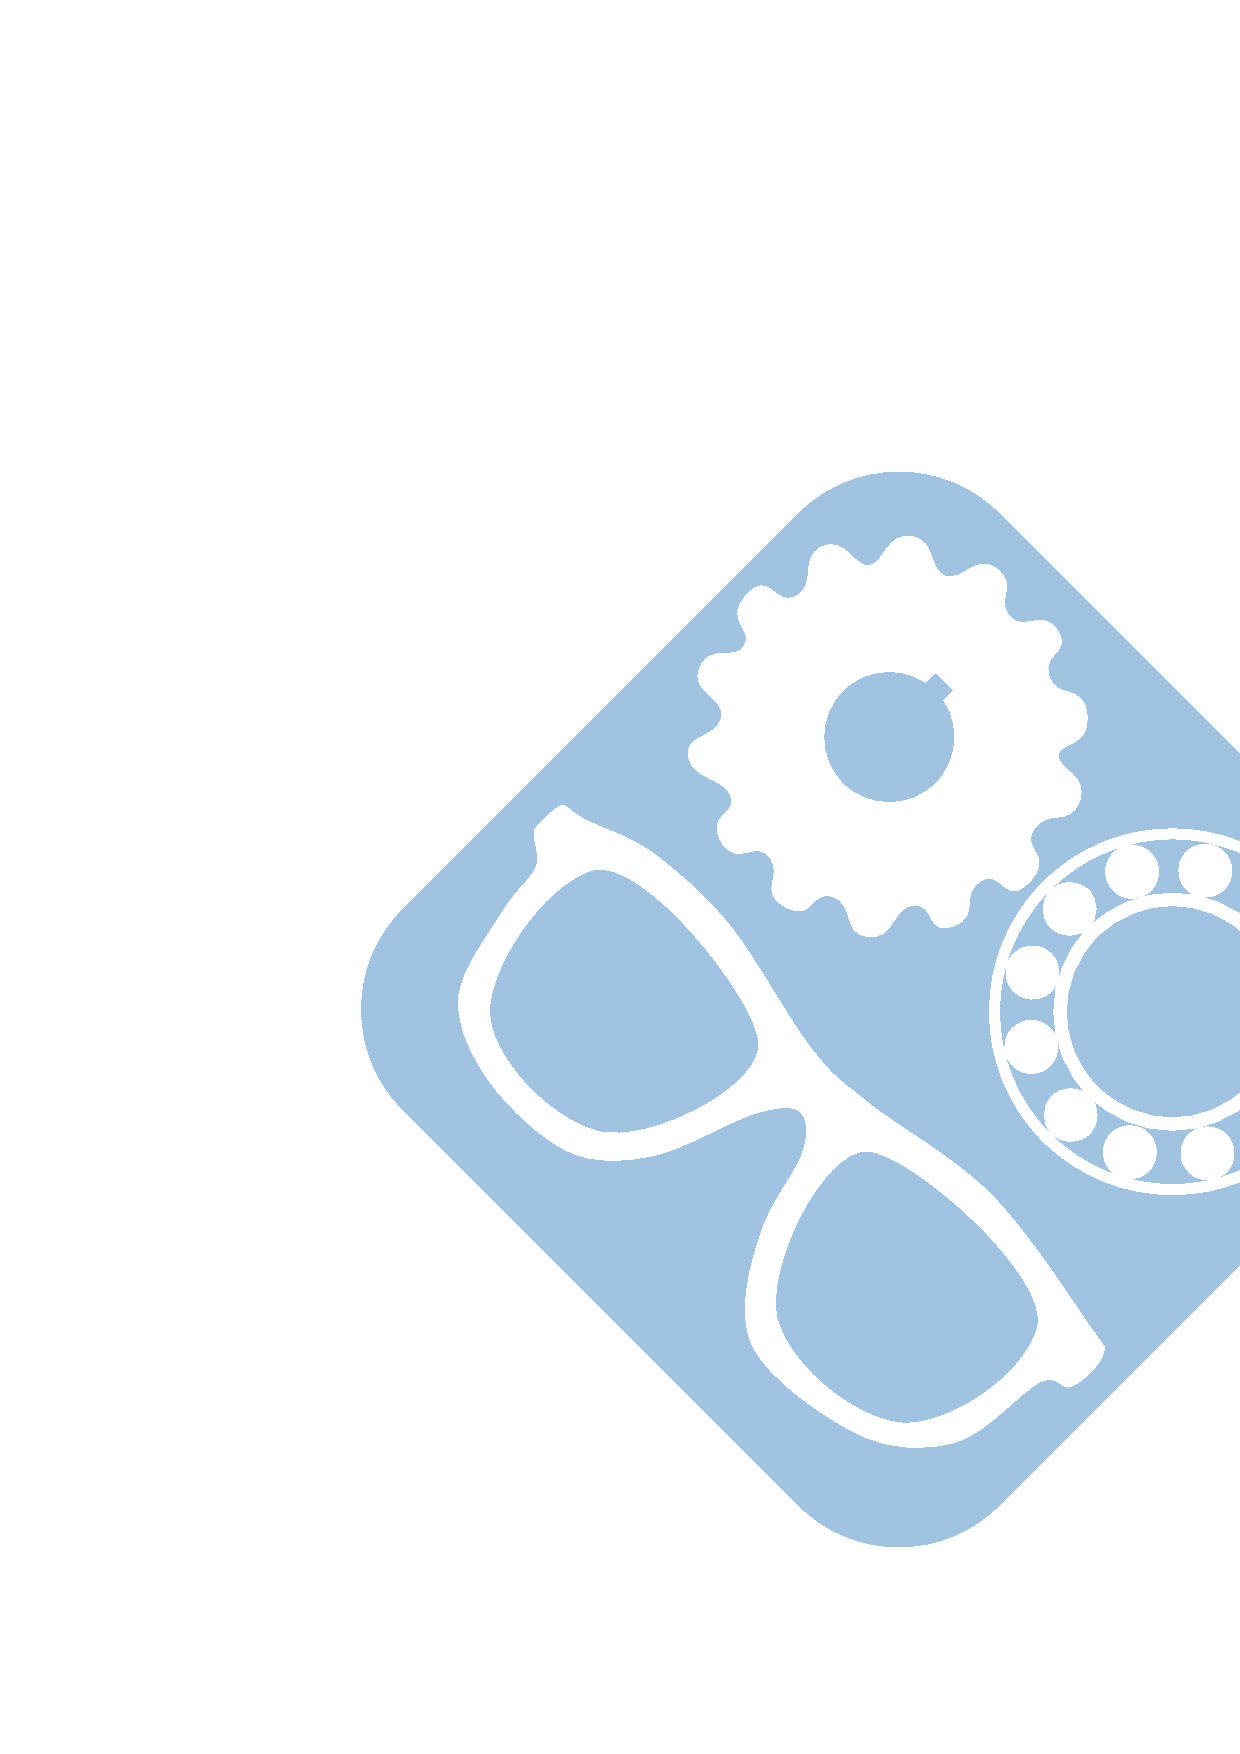
\includegraphics[width=\paperwidth,height=\paperheight,%
keepaspectratio]{../../img/fond3}%
\end{center}
\vfill
}}}

\newcommand{\BackgroundPicdeux}{%
\put(25,-30){%
\parbox[b][\paperheight]{\paperwidth}{%
\vfill
\begin{center}

\includegraphics[width=\paperwidth,height=\paperheight,%
keepaspectratio]{../../img/fond4}%
\end{center}
\vfill
}}}

\begin{document}

\pagestyle{empty}

\vspace*{-3\baselineskip}

\AddToShipoutPicture*{\BackgroundPic}

\ifdef{\auteurdeux}{\begin{tabular}{>{\columncolor{gray!00}}m{.3\linewidth} m{.3\linewidth} >{\columncolor{gray!00}}m{.3\linewidth}}
Séquence : \sequence &  \multirow{3}{*}{\hspace{1cm}
\includegraphics[height=1.5cm]{../../img/logo}} &  \begin{flushright} \multirow{4}{*}{\hspace{1cm}
\includegraphics[height=4cm]{img/qrcode}}\end{flushright}\\
Document : \type\num \\
 \institute \\
 \auteurun\\
 \auteurdeux
\end{tabular}}{\begin{tabular}{>{\columncolor{gray!00}}m{.3\linewidth} m{.3\linewidth} >{\columncolor{gray!00}}m{.3\linewidth}}
Séquence : \sequence &  \multirow{3}{*}{\hspace{1cm}
\includegraphics[height=1.5cm]{../../img/logo}} &  \begin{flushright} \multirow{4}{*}{\hspace{1cm}
\includegraphics[height=4cm]{img/qrcode}}\end{flushright}\\
Document : \type\num \\
 \institute \\
 \auteurun
\end{tabular}}

\vspace{1cm}

\ifdef{\prive}{\begin{center}\colorbox{danger}{\Huge{Avec Correction}}\end{center}}{}

\begin{center}\huge{\nom}\end{center}

\vspace{2cm}

\ifdef{\imagedeux}{\begin{minipage}{0.49\linewidth}}{}
\begin{center}\includegraphics[height=5cm]{/home/renaud/Documents/Renaud/GitHub/django_education/systemes/\imageun}\end{center}
\ifdef{\imagedeux}{\end{minipage}\hfill
\begin{minipage}{0.49\linewidth}
\begin{center}\includegraphics[height=5cm]{/home/renaud/Documents/Renaud/GitHub/django_education/systemes/\imagedeux}\end{center}
\end{minipage}}{}

\vspace{5cm}


\begin{tabular}{p{.15\linewidth} >{\columncolor{white}}p{.8\linewidth}}
    \rowcolor{gray!20}
    Référence & S\sequence\ - \type\num \\
    Compétences & \competences \\
 	\rowcolor{gray!20}
    Description & \descrip \\
    Système & \systemes
  \end{tabular}

\newpage

\AddToShipoutPicture{\BackgroundPicdeux}

\pagestyle{normal}

\section{Étude de chronogrammes}

\paragraph{Question 1:} Déduire du chronogramme la table de vérité de S 

~\

\begin{figure}[!h]
 \begin{minipage}{0.6\linewidth}
    \centering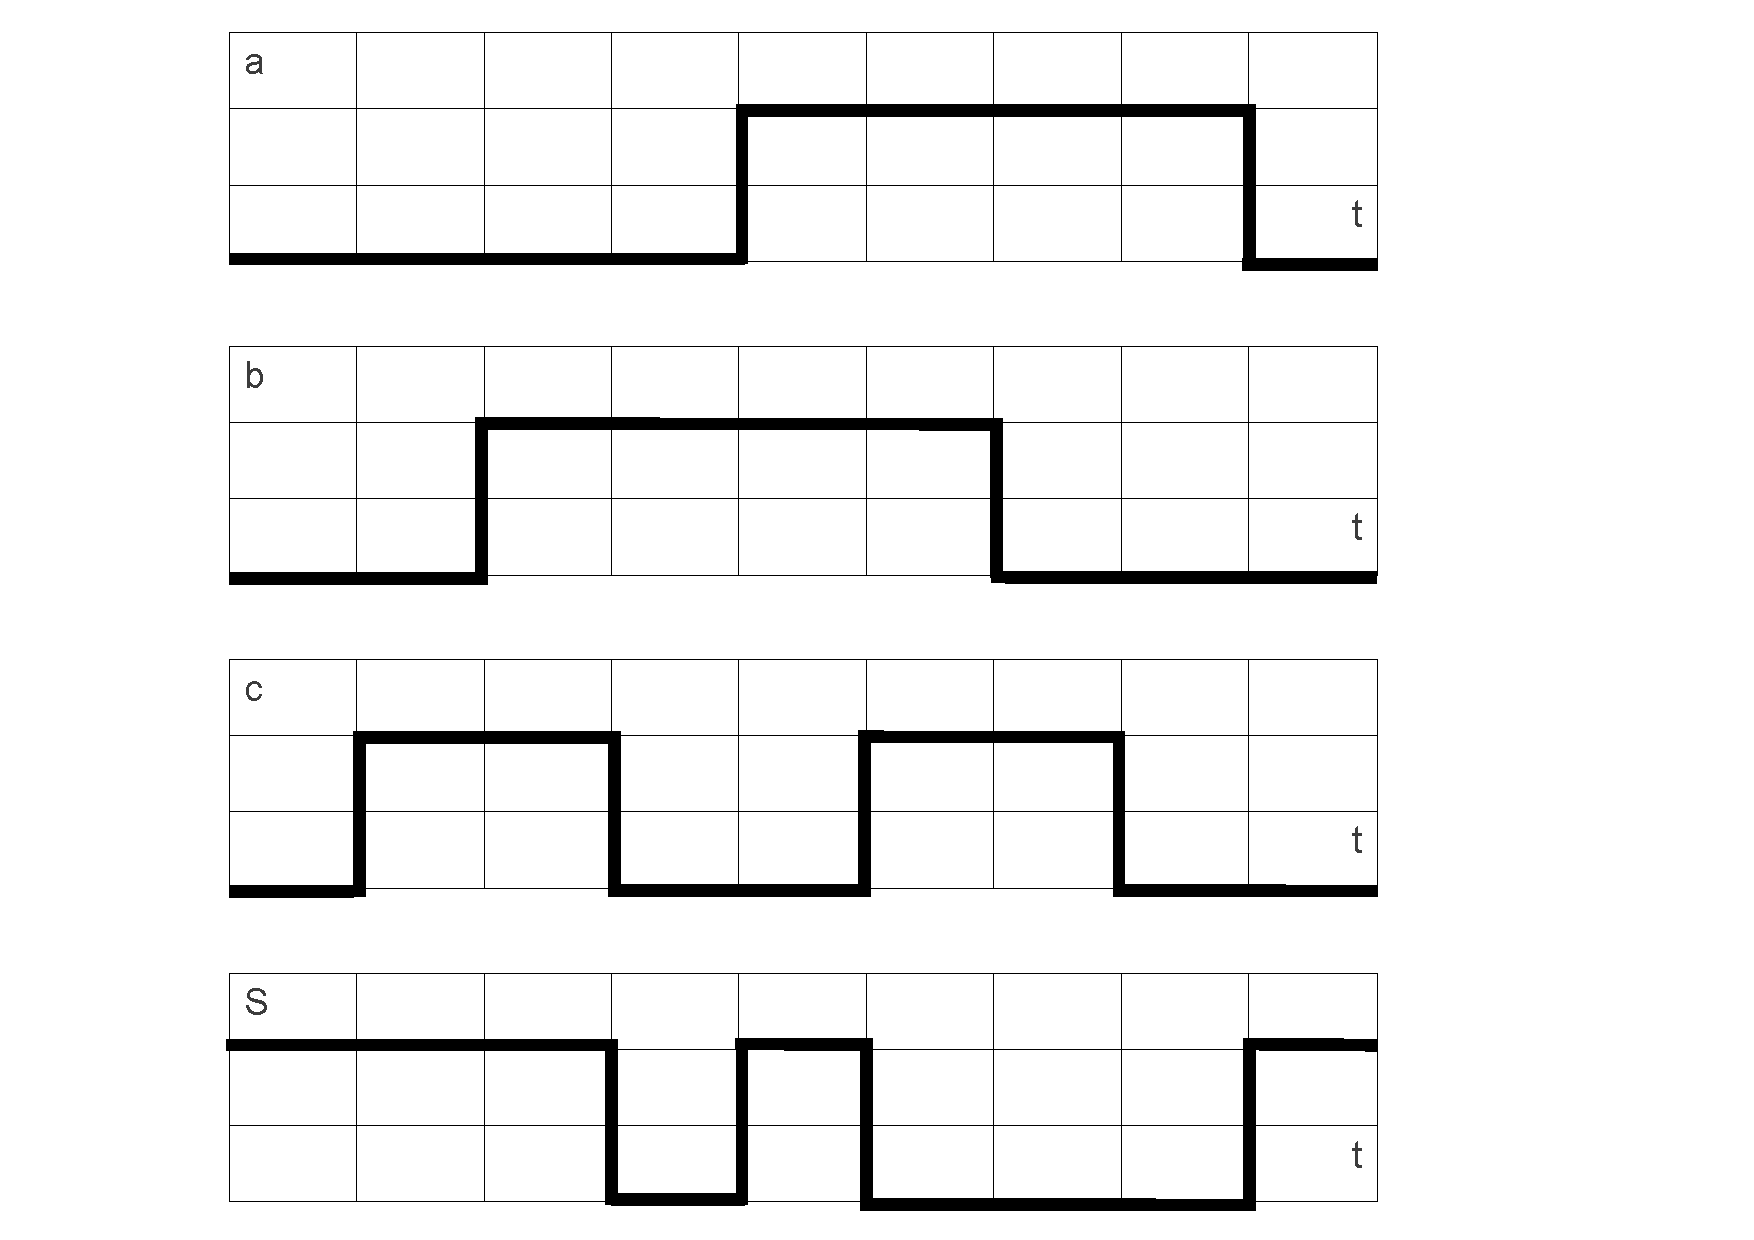
\includegraphics[width=1\linewidth]{img/chrono.pdf}
 \end{minipage}
 \hfill
 \begin{minipage}{0.38\linewidth}
 \begin{center}
 \begin{tabular}{|c|c|c|c|}
 \hline
 a & b & c & S \\
 \hline
   &   &   &   \\
 \hline
   &   &   &   \\
 \hline
   &   &   &   \\
 \hline
   &   &   &   \\
 \hline
   &   &   &   \\
 \hline
   &   &   &   \\
 \hline
   &   &   &   \\
 \hline
   &   &   &   \\
 \hline
 \end{tabular}
 \end{center}
 \end{minipage}
\end{figure}


\paragraph{Question 2:} Compléter le tableau de Karnaugh suivant et en déduire une forme simplifiée de $S$.

~\

\begin{center}
\begin{tabular}{|c|c|c|c|c|}
\hline
a $\backslash$ bc & 00 & 01 & 11 & 10 \\
\hline
0  &    &    &    &    \\
\hline
1  &    &    &    & \\
\hline
\end{tabular} 
\end{center}

\section{Système de transmission avec correction d'erreur}

Dans un système de transmission, il est souhaitable d'être capable de détecter et de corriger une erreur. Pour cela, il est possible d'utiliser un \og Code de Hamming\fg.

Pour transmettre les 4 éléments binaires $m_1$, $m_2$, $m_3$, $m_4$ correspondant à un chiffre du système décimal. 3 éléments binaires de contrôle $k_1$, $k_2$, $k_3$ sont ajoutés.

La position relative des éléments binaire est donnée dans le tableau suivant.

\begin{center}
\begin{tabular}{|c|c|c|c|c|c|c|c|}
\hline
n & 1 & 2 & 3 & 4 & 5 & 6 & 7 \\
\hline
  & $k_1$ & $k_2$ & $m_1$ & $k_3$ & $m_2$ & $m_3$ & $m_4$ \\
\hline
\end{tabular} 
\end{center}

3 tests de parité sont effectués pour détecter l'erreur:
\begin{itemize}
 \item test $T_1$ se fait sur les éléments binaires 1 3 5 7,
 \item test $T_2$ se fait sur les éléments binaires 2 3 6 7,
 \item test $T_3$ se fait sur les éléments binaires 4 5 6 7.
\end{itemize}

Le résultat d'un test de parité donne 0 si le nombre de 1 dans la zone considérée est pair.

\begin{center}
\begin{tabular}{|c|c|c|c|c|c|c|c|c|}
\hline
N  & $k_1$ & $k_2$ & $m_1$ & $k_3$ & $m_2$ & $m_3$ & $m_4$ \\
\hline
0 & 0 & 0 & 0 & 0 & 0 & 0 & 0 \\
\hline
1 & 1 & 1 & 0 & 1 & 0 & 0 & 1 \\
\hline
2 & 0 & 1 & 0 & 1 & 0 & 1 & 0 \\
\hline
3 & 1 & 0 & 0 & 0 & 0 & 1 & 1 \\
\hline
4 & 1 & 0 & 0 & 1 & 1 & 0 & 0 \\
\hline
5 & 0 & 1 & 0 & 0 & 1 & 0 & 1 \\
\hline
6 & 1 & 1 & 0 & 0 & 1 & 1 & 0 \\
\hline
7 & 0 & 0 & 0 & 1 & 1 & 1 & 1 \\
\hline
8 & 1 & 1 & 1 & 0 & 0 & 0 & 0 \\
\hline
9 & 0 & 0 & 1 & 1 & 0 & 0 & 1 \\
\hline
\end{tabular} 
\end{center}

La disposition est choisie de telle façon que le nombre binaire $(T_3T_2T_1)_2$ formé par les résultats des tests $T_1$ à $T_3$ donne la position de l'élément binaire ($k_i$,$m_i$) où se trouve l'erreur.

\paragraph{Question 1:} Effectuer les trois tests sur le résultat suivant.

\begin{center}
\begin{tabular}{|c|c|c|c|c|c|c|c|c|c|c|}
\hline
$k_1$ & $k_2$ & $m_1$ & $k_3$ & $m_2$ & $m_3$ & $m_4$ & $T_1$ & $T_2$ & $T_3$\\
\hline
1 & 0 & 0 & 1 & 0 & 0 & 0 & & & \\
\hline
\end{tabular} 
\end{center}

Où se trouve l'erreur, à quelle ligne du tableau initial cet envoi correspond-t-il?

\paragraph{Question 2:} Déterminer les fonctions logiques permettant de produire $k_1$, $k_2$, $k_3$. Montrer qu'un seul type de porte logique est utilisable. En déduire le schéma du dispositif émetteur de $k_1$.

\paragraph{Question 3:} Proposer les pistes de la réalisation du schéma du dispositif récepteur.

\section{Codeur incrémental}

La mesure de déplacement en rotation d'une vis et de sa vitesse est réalisée grâce à un capteur incrémental 500 points par tour.

Le schéma ci-dessous représente partiellement le disque du capteur incrémental et les 2 cellules photoélectriques CA et CB.

Ce disque comporte une piste où alternent zones opaques (noires sur le schéma) et zones transparentes (blanches que le schéma). Les cellules CA et CB renvoient un signal 0 ou 1 selon qu'elles se trouvent respectivement en face d'une zone opaque ou d'une zone transparente. Les 2 cellules CA et CB sont placées de telle manière que les signaux A et B qu'elles délivrent sont décalés d'un quart de période.

\begin{center}
 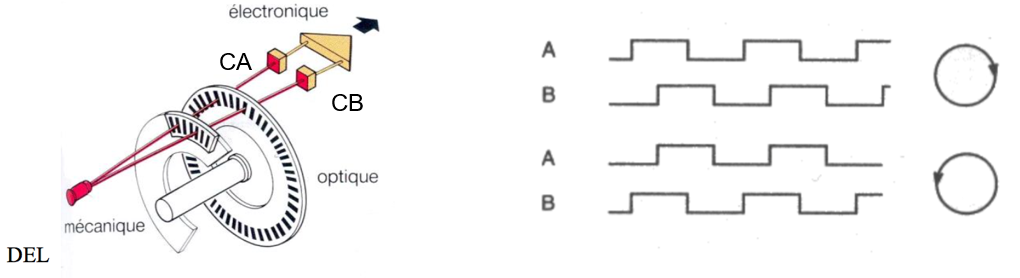
\includegraphics[width=0.7\linewidth]{img/figure01}
\end{center}

\paragraph{Question 1:} Donner l'état des signaux binaires A et B respectivement associés à CA et CB pour les zones a, b, c, d, e, f, g.

\begin{center}
 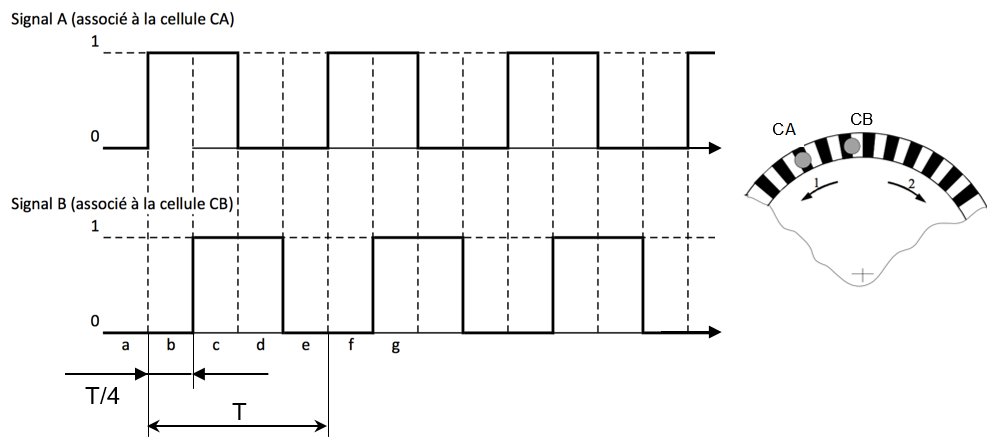
\includegraphics[width=0.7\linewidth]{img/figure02}
\end{center}

\paragraph{Question 2:} Le capteur incrémental utilisé sur la machine délivre 500 points par tour. Combien doit-il y avoir de couples de zones sur la piste du disque?

\paragraph{Question 3:} Le capteur incrémental est monté directement en bout de l'une des vis de déplacement de la traverse dont le pas est de 5 mm. Avec quelle précision peut-on connaître la position de la traverse ?

\paragraph{Question 4:} Une période correspond à l'intervalle T sur le schéma. L'intérêt de décaler les deux signaux d'un quart de période est de pouvoir détecter le sens de rotation du disque. Compte tenu de la forme proposée des signaux et de la position des deux cellules C1 et C2, dans quel sens le disque tourne-t-il (sens 1 ou 2, voir schéma du capteur incrémental en haut de page) ? Justifier la réponse. 

\begin{center}
 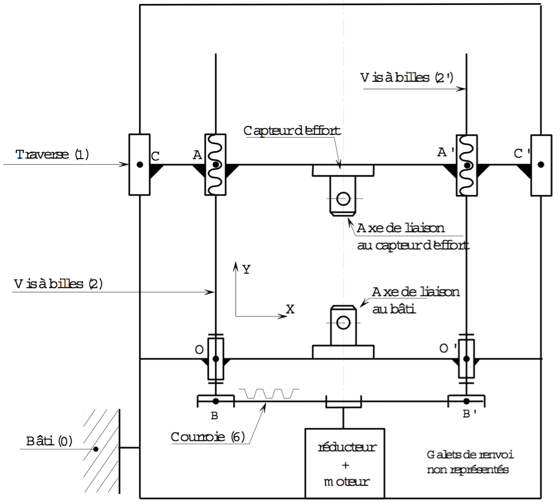
\includegraphics[width=0.6\linewidth]{img/figure05}
\end{center}

\section{Code à barres}

Le laboratoire utilisateur de la machine étudiée, réalise différents essais sur des éprouvettes de matériaux différents, provenant de fournisseurs différents. Pour un matériau, un fournisseur et un type d'essai donnés, on réalise 5 essais. Chaque éprouvette de l'essai est répertoriée par un code à barre composé de caractères alphanumériques propres à l'entreprise. Ce code renseigne sur le fournisseur (1 caractère), le matériau (1 caractère), l'essai (1 caractère) et le numéro de l'éprouvette (1 chiffre {1, 2, 3, 4, 5}).

Le code à barres retenu est le code \og 39 \fg, voir annexe 2. Ce code est constitué pour chaque caractère alphanumérique de 5 barres étroites ou larges et de 4 espaces étroits ou larges. Une barre étroite correspond à la valeur binaire 0, une large à la valeur 1. De même un espace étroit correspond à 0 et un large à 1. On code donc un caractère alphanumérique sur 9 digits (5 barres et 4 espaces) dont 3 sont à 1 et les autres à 0.

Les digits sont regroupés en deux mots, l'un, B, de 5 bits (correspondant aux 5 barres), l'autre, E, de 4 bits (correspondant aux 4 espaces). On associe de plus à chaque caractère alphanumérique un nombre X. Voir annexe 2.

Chaque code est constitué d'un espace, d'un caractère de début, \textbf{des caractères du code proprement dit}, d'un caractère de contrôle et d'un caractère de fin.

Le caractère de contrôle est tel que son nombre X est égal à la somme modulo 43 des nombres X \textbf{des caractères du code proprement dit}.

Pour ce qui suit, on ne tient pas compte des espaces et caractères de début et de fin. Le lecteur de code à barres renvoie pour une éprouvette le code figurant sur la figure ci-dessous.

\begin{center}
 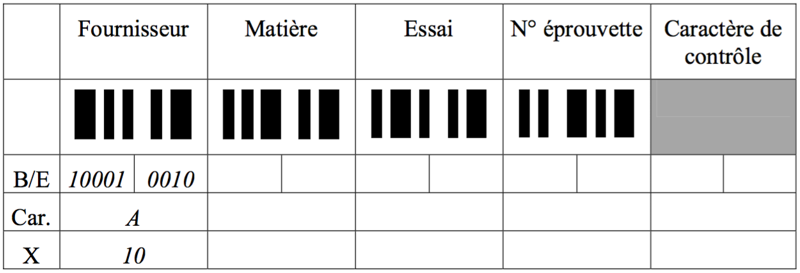
\includegraphics[width=0.7\linewidth]{img/figure03}
\end{center}

\paragraph{Question 1:} Compléter le tableau figurant sur la feuille réponse. Donner pour chaque code à barres et pour le caractère de contrôle les mots B et E. le caractère alphanumérique correspondant et la valeur de X. 

On s'intéresse maintenant au transcodeur permettant de passer pour les numéros d'éprouvette du code "39" au code binaire naturel. 
Les seuls chiffres utilisés pour le numéro de l'éprouvette sont 1, 2, 3, 4 et 5. 

\paragraph{Question 2:} Combien un mot, en binaire naturel, doit-il comporter de bits pour coder les chiffres de 1 à 5 ? 

On note $B=b_4b_3b_2b_1b_0$, $E=e_3e_2e_1e_0$ et $N=n_nn_{n-1}...n_1n_0$ le mot binaire naturel.

\paragraph{Question 3:} Donner les équations de $n_n$, $n_{n-1}$,...,$n_1$, $n_0$ en fonction des $b_i$ et $e_i$. (Tous les $b_i$ et $e_i$ n'interviennent pas forcément). 

\begin{center}
 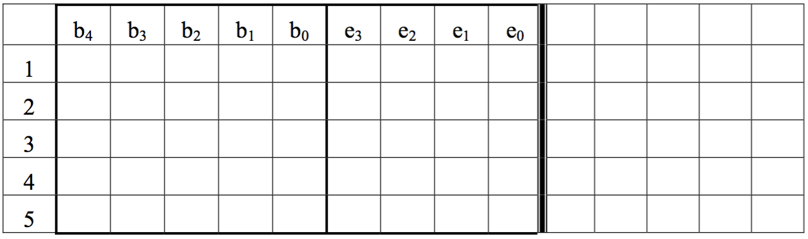
\includegraphics[width=0.7\linewidth]{img/figure04}
\end{center}


\begin{center}
Annexe 2 \\
 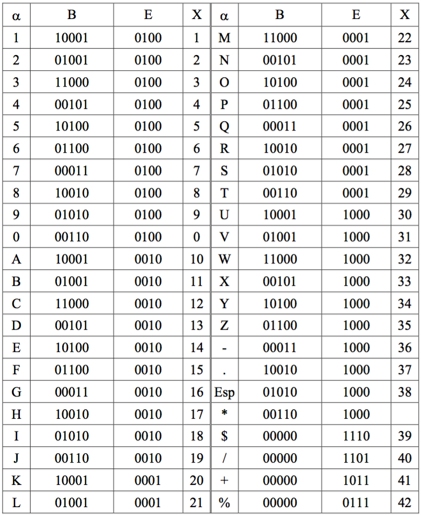
\includegraphics[width=0.6\linewidth]{img/figure06}
\end{center}

\section{Conversion de nombre}

\paragraph{Question 1:}

Convertir, $(010011)_{2}$:
\begin{itemize}
 \item en décimal,
 \item en octal,
 \item en hexadécimal.
\end{itemize}

\paragraph{Question 2:}

Convertir le nombre suivant $(145)_{10}$ en binaire.

\paragraph{Question 3:}

Convertir, $(746)_{8}$ en binaire.

\paragraph{Question 4:}

Convertir, $(A35F)_{16}$ en binaire.

\section{Opérations sur les nombres binaires}

\paragraph{Question 1:}

Calculer, $(010110)_{2}+(110100)_{2}$.

~\

\paragraph{Question 2:}

Calculer, $(110100)_{2}-(001010)_{2}$.

~\

\paragraph{Question 3:}

Calculer, $(10010)_{2}*(101)_{2}$.

~\

\paragraph{Question 4:}

Calculer, $\frac{(11110)_{2}}{(110)_{2}}$.

~\

\section{Opérateur OU Exclusif}

\paragraph{Question 1:}

Développer sous la forme canonique $S= a \oplus b \oplus c$.

\paragraph{Question 2:}

Représenter sous la forme d'un tableau de Karnaugh

~\

\begin{center}
\begin{tabular}{|c|c|c|c|c|}
\hline
ab & 00 & 01 & 11 & 10 \\
\hline
0  &    &    &    &    \\
\hline
1  &    &    &    & \\
\hline
\end{tabular} 
\end{center}

\paragraph{Question 3:}

Déterminer $\overline{S}$.

\clearpage

\ifdef{\public}{\end{document}}{}

\newpage

\pagestyle{correction}

\section{Correction}

\subsection{Étude de chronogramme}

\paragraph{Question 1:}

 \begin{center}
 \begin{tabular}{|c|c|c|c|}
 \hline
 a & b & c & S \\
 \hline
 0  & 0  & 0  & 1 \\
 \hline
 0  & 0  & 1  & 1 \\
 \hline
 0  & 1  & 0  & 0 \\
 \hline
 0  & 1  & 1  & 1 \\
 \hline
 1  & 0  & 0  & 0 \\
 \hline
 1  & 0  & 1  & 0 \\
 \hline
 1  & 1  & 0  & 1 \\
 \hline
 1  & 1  & 1  & 0 \\
 \hline
 \end{tabular}
 \end{center}

\paragraph{Question 2:}

\begin{center}
\begin{tabular}{|c|c|c|c|c|}
\hline
a $\backslash$ bc & 00 & 01 & 11 & 10 \\
\hline
0  & 1 & 1 & 1 & 0 \\
\hline
1  & 0 & 0 & 0 & 1 \\
\hline
\end{tabular} 
\end{center}

\subsection{Système de transmission}

\paragraph{Question 1:} $(T_3T_2T_1)_2=(101)_2=5$, l'erreur est sur la colonne 5.

\paragraph{Question 2:} ~\

\begin{minipage}{0.45\linewidth}
\begin{center}
\begin{tabular}{|c|c|c|c|c|}
\hline
\multicolumn{5}{|c|}{$k_1$} \\
\hline
$m_1$ $m_2$ $\backslash$ $m_3$ $m_4$ & 00 & 01 & 11 & 10 \\
\hline
00  & 0 & \cellcolor{bleuf} 1 & \cellcolor{bleuf} 1 & 0 \\
\hline
01  & \cellcolor{bleuf}1 & 0 & 0 &  \cellcolor{bleuf} 1 \\
\hline
11  & \cellcolor{bleuf} &  &  & \cellcolor{bleuf} \\
\hline
10  & \cellcolor{bleuf} 1 & 0 &  & \cellcolor{bleuf} \\
\hline
\end{tabular} 
\end{center}
\end{minipage}\hfill
\begin{minipage}{0.45\linewidth}
$k_1=m_2.\overline{m_4}+m_1.\overline{m_4}+\overline{m_1}.\overline{m_2}.m_4$
\end{minipage}

\begin{minipage}{0.45\linewidth}
\begin{center}
\begin{tabular}{|c|c|c|c|c|}
\hline
\multicolumn{5}{|c|}{$k_2$} \\
\hline
$m_1$ $m_2$ $\backslash$ $m_3$ $m_4$ & 00 & 01 & 11 & 10 \\
\hline
00  & 0 & \cellcolor{bleuf} 1 & 0 & \cellcolor{bleuf} 1  \\
\hline
01  & 0 & \cellcolor{bleuf} 1 & 0 &  \cellcolor{bleuf} 1 \\
\hline
11  & \cellcolor{bleuf} &  &  & \cellcolor{bleuf} \\
\hline
10  & \cellcolor{bleuf} 1 & 0 &  & \cellcolor{bleuf} \\
\hline
\end{tabular} 
\end{center}
\end{minipage}\hfill
\begin{minipage}{0.45\linewidth}
$k_2=m_3.\overline{m_4}+m_1.\overline{m_4}+\overline{m_1}.\overline{m_3}.m_4$
\end{minipage}

\begin{minipage}{0.45\linewidth}
\begin{center}
\begin{tabular}{|c|c|c|c|c|}
\hline
\multicolumn{5}{|c|}{$k_2$} \\
\hline
$m_1$ $m_2$ $\backslash$ $m_3$ $m_4$ & 00 & 01 & 11 & 10 \\
\hline
00  & 0 & \cellcolor{bleuf} 1 & 0 & \cellcolor{bleuf} 1  \\
\hline
01  & 0 & \cellcolor{bleuf} 1 & 0 &  \cellcolor{bleuf} 1 \\
\hline
11  & \cellcolor{bleuf} &  & \cellcolor{bleuf} &  \\
\hline
10  & \cellcolor{bleuf} 1 & 0 & \cellcolor{bleuf} &  \\
\hline
\end{tabular} 
\end{center}
\end{minipage}\hfill
\begin{minipage}{0.45\linewidth}
$k_2=(m_1 \oplus m_3) \oplus m_4$
\end{minipage}

\begin{minipage}{0.45\linewidth}
\begin{center}
\begin{tabular}{|c|c|c|c|c|}
\hline
\multicolumn{5}{|c|}{$k_3$} \\
\hline
$m_1$ $m_2$ $\backslash$ $m_3$ $m_4$ & 00 & 01 & 11 & 10 \\
\hline
00  & 0 & \cellcolor{bleuf} 1 & 0 & \cellcolor{bleuf} 1 \\
\hline
01  & \cellcolor{bleuf}1 & 0 &  \cellcolor{bleuf} 1 & 0 \\
\hline
11  & \cellcolor{bleuf}1 &   & \cellcolor{bleuf} &  \\
\hline
10  & 0 & \cellcolor{bleuf} 1 &  & \cellcolor{bleuf}  \\
\hline
\end{tabular} 
\end{center}
\end{minipage}\hfill
\begin{minipage}{0.45\linewidth}
$k_3=m_2.\overline{m_3}.\overline{m_4}+.\overline{m_2}.\overline{m_3}.m_4+m_2.m_3.m_4+\overline{m_2}.m_3.\overline{m_4}=(m_2 \oplus m_3) \oplus m_4$
\end{minipage}

\paragraph{Question 3:}

$k_1=m_2.\overline{m_4}+m_1.\overline{m_4}+\overline{m_1}.\overline{m_2}.m_4$

Donc, $\overline{k_1}=\overline{(m_1+m_2).\overline{m_4}}.\overline{\overline{m_1}.\overline{m_2}.m_4}=\overline{\overline{\overline{m_1}.\overline{m_2}}.\overline{m_4}}.\overline{\overline{m_1}.\overline{m_2}.m_4}$

\begin{center}
 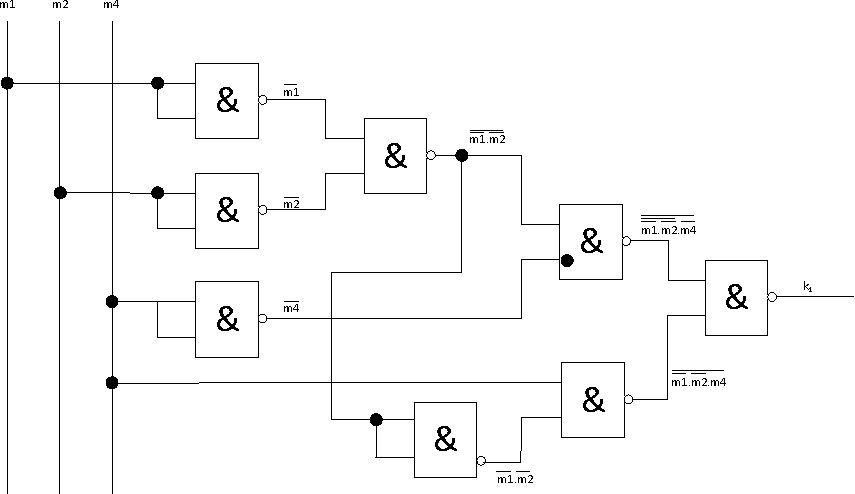
\includegraphics[width=0.8\linewidth]{img/nands}
\end{center}
\subsection{Codeur incrémental}

\paragraph{Question 1:} Donner l'état des signaux binaires A et B respectivement associés à CA et CB pour les zones a, b, c, d, e, f, g.

\begin{center}
\begin{tabular}{|c|c|c|c|c|c|c|c|}
\hline
  & a & b & c & d & e & f & g \\
\hline
A & 0 & 1 & 1 & 0 & 0 & 1 & 1 \\
\hline
B & 0 & 0 & 1 & 1 & 0 & 0 & 1 \\
\hline
\end{tabular}
\end{center}

\paragraph{Question 2:} Le capteur incrémental utilisé sur la machine délivre 500 points par tour. Combien doit-il y avoir de couples de zones sur la piste du disque?

Deux informations par couple blanc/noir par cellule, cela signifie $\frac{500}{4}=125 couples$.

\paragraph{Question 3:} Le capteur incrémental est monté directement en bout de l'une des vis de déplacement de la traverse dont le pas est de 5 mm. Avec quelle précision peut-on connaître la position de la traverse ?

$\frac{5}{500}=0.01mm$

\paragraph{Question 4:} Une période correspond à l'intervalle T sur le schéma. L'intérêt de décaler les deux signaux d'un quart de période est de pouvoir détecter le sens de rotation du disque. Compte tenu de la forme proposée des signaux et de la position des deux cellules C1 et C2, dans quel sens le disque tourne-t-il (sens 1 ou 2, voir schéma du capteur incrémental en haut de page) ? Justifier la réponse. 

Il s'agit du sens horaire, sens 2.

\subsection{Code à barres}

\paragraph{Question 1:} Compléter le tableau figurant sur la feuille réponse. Donner pour chaque code à barres, et pour le caractère de contrôle les mots B et E, le caractère alphanumérique correspondant et la valeur de X. 

\begin{center}
\begin{tabular}{|c|c|c|c|c|c|c|c|c|c|c|}
\hline
B/E & 10001 & 0010 & 00101 & 0010 & 01001 & 0010 & 00101 & 0100 & 01010 & 1000 \\
\hline
Car & \multicolumn{2}{c|}{A} & \multicolumn{2}{c|}{D} & \multicolumn{2}{c|}{B} & \multicolumn{2}{c|}{4} & \multicolumn{2}{c|}{ESP} \\
\hline
X & \multicolumn{2}{c|}{10} & \multicolumn{2}{c|}{13} & \multicolumn{2}{c|}{11} & \multicolumn{2}{c|}{4} & \multicolumn{2}{c|}{38} \\
\hline
\end{tabular}
\end{center}

\paragraph{Question 2:} Combien un mot, en binaire naturel, doit-il comporter de bits pour coder les chiffres de 1 à 5 ? 

Il faut 3 bits.

\paragraph{Question 3:} Donner les équations de $n_n$, $n_{n-1}$,...,$n_1$, $n_0$ en fonction des $b_i$ et $e_i$. (Tous les $b_i$ et $e_i$ n'interviennent pas forcément). 

\begin{center}
\begin{tabular}{|c|c|c|c|c|c|c|c|c|c||c|c|c|}
\hline
 & $b_4$ & $b_3$ & $b_2$ & $b_1$ & $b_0$ & $e_3$ & $e_2$ & $e_1$ & $e_0$ & $n_2$ & $n_1$ & $n_0$ \\
\hline
1 & 1 & 0 & 0 & 0 & 1 & 0 & 1 & 0 & 0 & 0 & 0 & 1\\
\hline
2 & 0 & 1 & 0 & 0 & 1 & 0 & 1 & 0 & 0 & 0 & 1 & 0\\
\hline
3 & 1 & 1 & 0 & 0 & 0 & 0 & 1 & 0 & 0 & 0 & 1 & 1\\
\hline
4 & 0 & 0 & 1 & 0 & 1 & 0 & 1 & 0 & 0 & 1 & 0 & 0\\
\hline
5 & 1 & 0 & 1 & 0 & 0 & 0 & 1 & 0 & 0 & 1 & 0 & 1 \\
\hline
\end{tabular}
\end{center}

$n_0=b_4$, $n_1=b_3$, $n_2=b_2$.

\subsection{Conversion de nombre}

\paragraph{Question 1:}

Convertir, $(010011)_{2}$:
\begin{itemize}
 \item en décimal: $19_{10}$,
 \item en octal: $23_{8}$,
 \item en hexadécimal: $13_{16}$.
\end{itemize}

\paragraph{Question 2:}

Convertir le nombre suivant $(145)_{10}$ en binaire.

$(10010001)_{2}$

\paragraph{Question 3:} Convertir, $(746)_{8}$ en binaire.

$(111100110)_{2}$

\paragraph{Question 4:} Convertir, $(A35F)_{16}$ en binaire.

1010001101011111

\subsection{Opérations sur les nombres binaires}

\paragraph{Question 1:}

Calculer, $(010110)_{2}+(110100)_{2}$.

1001010

~\

\paragraph{Question 2:}

Calculer, $(110100)_{2}-(001010)_{2}$.

$(101010)_{2}$

~\

\paragraph{Question 3:}

Calculer, $(10010)_{2}*(101)_{2}$.

$(1011010)_{2}$

~\

\paragraph{Question 4:}

Calculer, $\frac{(11110)_{2}}{(110)_{2}}$.

$(101)_{2}$

~\

\subsection{Opérateur OU Exclusif}

\paragraph{Question 1:}

Développer sous la forme canonique $S= a \oplus b \oplus c$.

$S= a \oplus b \oplus c=(\overline{a}.b+a.\overline{b}) \oplus c$

$S=(a.\overline{b}+\overline{a}.b).\overline{c}+\overline{(a.\overline{b}+\overline{a}.b)}.c$

$S=a.\overline{b}.\overline{c}+\overline{a}.b.\overline{c}+\overline{a}.\overline{b}.c+a.b.c$



\paragraph{Question 2:}

Représenter sous la forme d'un tableau de Karnaugh

~\

\begin{center}
\begin{tabular}{|c|c|c|c|c|}
\hline
a $\backslash$ bc & 00 & 01 & 11 & 10 \\
\hline
0  & 0 & 1 & 0 & 1 \\
\hline
1  & 1 & 0 & 1 & 0 \\
\hline
\end{tabular} 
\end{center}

\paragraph{Question 3:}

Déterminer $\overline{S}= \overline{a} \oplus \overline{b} \oplus \overline{c}$

\end{document}
